\begin{comment}
\documentclass[10pt]{article}
\usepackage{fullpage, graphicx, url}
\setlength{\parskip}{1ex}
\setlength{\parindent}{0ex}
\title{FLpack}
\begin{document}


\begin{tabular}{ccc}
The Alternative Csound Reference Manual & & \\
Previous & &Next

\end{tabular}

%\hline 
\end{comment}
\section{FLpack}
FLpack�--� Provides the functionality of compressing and aligning FLTK widgets. \subsection*{Description}


 \emph{FLpack}
 provides the functionality of compressing and aligning widgets. 
\subsection*{Syntax}


 \textbf{FLpack}
 iwidth, iheight, ix, iy, itype, ispace, iborder
\subsection*{Initialization}


 \emph{iwidth}
 -- width of widget. 


 \emph{iheight}
 -- height of widget. 


 \emph{ix}
 -- horizontal position of upper left corner of the valuator, relative to the upper left corner of corresponding window (expressed in pixels). 


 \emph{iy}
 -- vertical position of upper left corner of the valuator, relative to the upper left corner of corresponding window (expressed in pixels). 


 \emph{itype}
 -- an integer number that modifies the appearance of the target widget. 


  The \emph{itype}
 argument expresses the type of packing: 


 
\begin{itemize}
\item 

 0 - vertical

\item 

 1 - horizontal


\end{itemize}


 \emph{ispace}
 -- sets the space between the widgets. 


 \emph{iborder}
 -- border type of the container. It is expressed by means of an integer number chosen from the following: 


 
\begin{itemize}
\item 

 0 - no border

\item 

 1 - down box border

\item 

 2 - up box border

\item 

 3 - engraved border

\item 

 4 - embossed border

\item 

 5 - black line border

\item 

 6 - thin down border

\item 

 7 - thin up border


\end{itemize}
\subsection*{Performance}


 \emph{FLpack}
 provides the functionality of compressing and aligning widgets. 


  Containers are useful to format the graphic appearance of the widgets. The most important container is \emph{FLpanel}
, that actually creates a window. It can be filled with other containers and/or valuators or other kinds of widgets. 


  There are no k-rate arguments in containers. 
\subsection*{Examples}


  The following example: 


 
\begin{lstlisting}
        FLpanel "Panel1",450,300,100,100
        FLpack  400,300, 10,40,0,15,3
gk1,ihs1        FLslider        "FLslider 1", 500, 1000, 2 ,1, -1, 300,15, 20,50
gk2,ihs2        FLslider        "FLslider 2", 300, 5000, 2 ,3, -1, 300,15, 20,100
gk3,ihs3        FLslider        "FLslider 3", 350, 1000, 2 ,5, -1, 300,15, 20,150
gk4,ihs4        FLslider        "FLslider 4", 250, 5000, 1 ,11, -1, 300,30, 20,200
gk5,ihs5        FLslider        "FLslider 5", 220, 8000, 2 ,1, -1, 300,15, 20,250
gk6,ihs6        FLslider        "FLslider 6", 1, 5000, 1 ,13, -1, 300,15, 20,300
gk7,ihs7        FLslider        "FLslider 7", 870, 5000, 1 ,15, -1, 300,30, 20,350
        FLpackEnd
        FLpanelEnd
        
\end{lstlisting}


 
 ...will produce this result, when resizing the window: 

 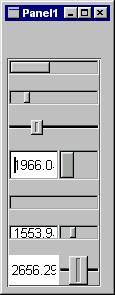
\includegraphics[scale=1]{flpack} 


 FLpack.
\subsection*{See Also}


 \emph{FLgroup}
, \emph{FLgroupEnd}
, \emph{FLpackEnd}
, \emph{FLpanel}
, \emph{FLpanelEnd}
, \emph{FLscroll}
, \emph{FLscrollEnd}
, \emph{FLtabs}
, \emph{FLtabsEnd}

\subsection*{Credits}


 Author: Gabriel Maldonado


 New in version 4.22
%\hline 


\begin{comment}
\begin{tabular}{lcr}
Previous &Home &Next \\
FLloadsnap &Up &FLpackEnd

\end{tabular}


\end{document}
\end{comment}
